\documentclass[10pt,paper=letter]{scrartcl}
\usepackage[alttitle]{cjquines}

\begin{document}

\title{VCSMS PRIME}
\subtitle{Program for Inducing Mathematical Excellence}
\author{Session 6: Circles and Polygons}
\date{September 29, 2017}

\maketitle
\setlength{\unitlength}{1in}
\begin{picture}(0,0)
  \put(5.5,0.5){\hbox{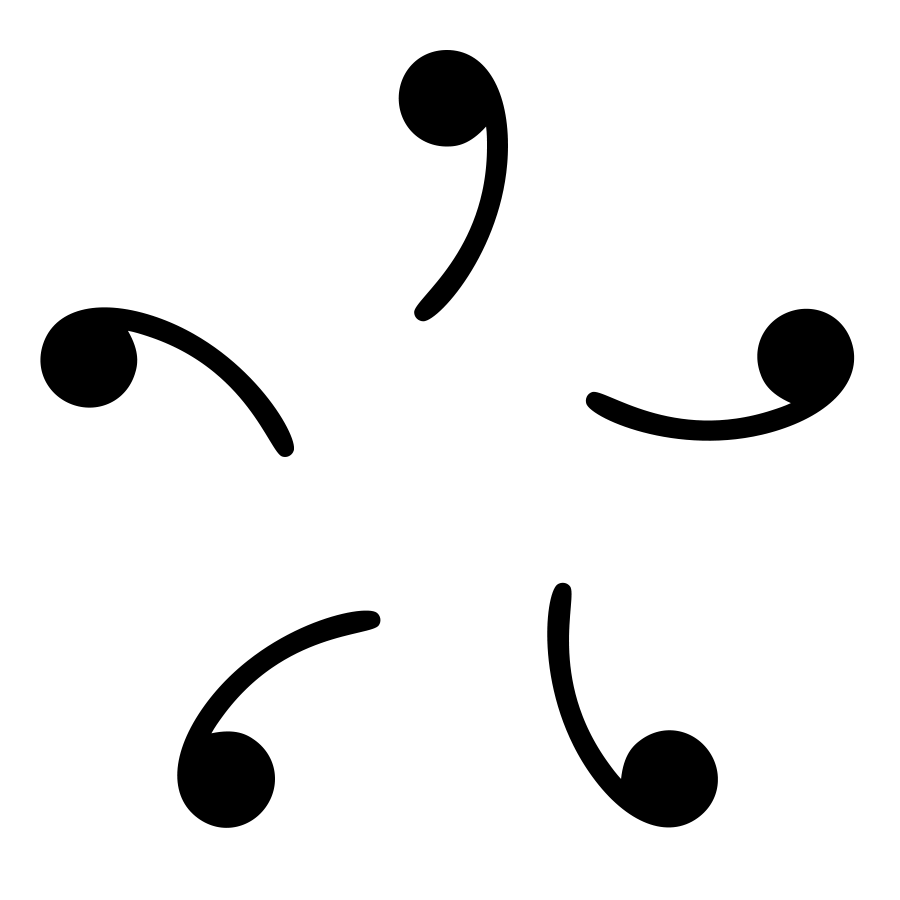
\includegraphics[width=0.9in]{logo.png}}}
\end{picture}
\vspace{-3.5em}

\subsubsection*{Lecture problems}

\begin{enumerate}
  \item (AI3) Let $O$ be the circumcenter of acute triangle $ACD$. The tangent to the circumcircle at $A$ intersects line $CO$ at $B$. If $AB||CD$, $AB = 6$ and $BC = 12$, what is the length of $CD$?
  \item (QI5) The sides of a triangle are $3$, $5$ and $x$. The sides of another triangle are $4$, $6$ and $y$. If the sides of both triangles are integers, what is the maximum value of $\abs{x - y}$?
  \item Two poles of heights $x$ and $y$ are perpendicular to the ground. A rope is tied from the top of the first to the bottom of the second, and another rope is tied from the top of the second to the bottom of the first. The two ropes intersect at a point that is distance $z$ from the ground. Show $1/x + 1/y = 1/z$.
  \item A square is inscribed in triangle $ABC$ such that two vertices lie on side $BC$, one vertex lies on $AB$, and the remaining vertex lies on $AC$. If $AB = 6$, $BC = 7$, and $CA = 8$, find the area of the square.
  \item A point $P$ and a rectangle $ABCD$ satisfy $AP = 7$, $BP = 5$, and $CP = 8$. Find $DP$.
  \item (QI3) One diagonal of a rhombus is three times as long as the other. If the rhombus has an area of $54$ square meters, what is its perimeter?
  \item (AI5) In parallelogram $ABCD$, $AB = 1$, $BC = 4$, and $\angle ABC = 60\dg$. Supose that $AC$ is extended from $A$ to a point $E$ beyond $C$ so that $ADE$ has the same area as the parallelogram. Find the length of $DE$.
  \item The diagonals in trapezoid $ABCD$ with $AB||CD$ intersect at point $E$. Given that $[ABE] = 25$ and $[CDE] = 64$, find $[ABCD]$.
  \item A quadrilateral circumscribed about a circle has side lengths $1, 2, 3, x$ in order. Find $x$.
  \item Two regular pentagons $WORLD$ and $LAYER$ are constructed outside each other. Find the length of $RL$ given $[ODAE] = \sqrt5$.
\end{enumerate}

\subsubsection*{Circles}

\begin{itemize}
  \item The perpendicular bisector of a chord is a diameter. Power of a point: If chords $AB$ and $CD$ intersect internally at $P$ (if $P$ lies outside the circle it must be closer to $A$ than $B$, and to $C$ than $D$), then $AP \cdot BP = CP \cdot DP$.
  \item Problem 1: Let $AO$ intersect $CD$ at $E$. Then $\triangle COE \sim \triangle BOA$, use power of a point.
  \item We can find lengths of common external and internal tangents given distance of centers and radii.
\end{itemize}

\subsubsection*{Triangles}

\begin{itemize}
  \item Problem 2: By triangle inequality, $2 < x < 8$ and $2 < y < 10$. Largest difference when $x = 3, y = 9$.
  \item All you have to do is find similar triangles! Example: altitude of a right triangle in terms of $a, b, c$.
  \item Problem 3: Look at the bases. Add up ratios: $z/x + z/y = 1$. This comes up a lot.
\end{itemize}

\subsubsection*{Squares}

\begin{itemize}
  \item Problem 4: Divide the area of the triangle into the area above the square, the area of the square, and the area to the left and right of the square. You get side length of square as $bh/(b+h)$.
\end{itemize}

\subsubsection*{Rectangles}

\begin{itemize}
  \item A parallelogram with congruent diagonals, or one right angle. 
  \item Problem 5: British Flag Theorem states that $AP^2 + CP^2 = BP^2 + DP^2$.
\end{itemize}

\subsubsection*{Rhombi}

\begin{itemize}
  \item A quadrilateral with all sides the same length. Its diagonals meet at right angles.
  \item Problem 6: Let diagonals be $6x$ and $2x$, its area is $6x \cdot 2x / 2$. Then by Pythagorean, a side is $\sqrt{(3x)^2 + x^2}$.
\end{itemize}

\subsubsection*{Parallelograms}

\begin{itemize}
  \item A quadrilateral whose opposite sides are parallel. Also, a quadrilateral whose diagonals bisect each other. Also, a quadrilateral whose pairs of opposite sides are the same length. Lots of congruent triangles. 
  \item Parallelogram law: sum of the squares of the sides is equal to sum of the squares of the diagonals.
  \item Problem 7: The area of $ADE$ is twice the area of $ACD$, but they both have the same height, so $AE$ is twice $AC$. Use law of cosines and Stewart's theorem.
\end{itemize}

\subsubsection*{Trapezoids}

\begin{itemize}
  \item A quadrilateral with \emph{at least} (sometimes exactly) one pair of opposite sides.
  \item If $AB||CD$ and $AD, BC$ intersect at $E$, then $\triangle ABE \sim \triangle DCE$ and $[AED] = [BEC]$. The segment connecting the midpoints of $AC$ and $BD$ passes through the midpoints of the diagonals and has length $(AB+CD)/2$. The segment connecting midpoints of diagonals has length $\abs{AB - CD}/2$.
  \item A trapezoid is isosceles iff it is cyclic. If you have a cyclic quadrilateral with congruent opposite sides, then it's automatically a trapezoid.
  \item Problem 8: From $[ABE][CDE] = [AED][BEC]$ (which is true for any quadrilateral) and $[AED] = [BEC]$ we can get the answer. Generally $\sqrt{[ABCD]} = \sqrt{[ABE]} + \sqrt{[CDE]}$ for any trapezoid.
\end{itemize}

\subsubsection*{Quadrilaterals}

\begin{itemize}
  \item The quadrilateral joining the midpoints of the sides is a parallelogram, and has half the area.
  \item The diagonals $AC$ and $BD$ are perpendicular iff $AB^2 + CD^2 = BC^2 + DA^2$. Then $[ABCD] = AC \cdot BD / 2$.
  \item If cyclic, area is $\sqrt{(s-a)(s-b)(s-c)(s-d)}$. This is Brahmagupta's formula.
\end{itemize}

\subsubsection*{Tangential polygons}

\begin{itemize}
  \item Use the fact that the tangents to the same circle from the same point are the same length. Example: tangent lengths to the incircle. Another: can a pentagon with side lengths $2, 3, 4, 5, 6$ be tangential?
  \item Problem 9: By Pitot's theorem, $1 + 3 = x + 2$, so $x = 2.$
\end{itemize}

\subsubsection*{Polygons}

\begin{itemize}
  \item Polygon inequality: any side of a polygon has to be less than the sum of the other sides. If this is satisfied, you can imagine it as a wireframe and can shift it to force a lot of things.
  \item Don't forget MMC: how many diagonals in an $n$-gon? Angle of regular $n$-gon?
  \item Problem 10: I told you the trigonometric functions of $36\dg$ were important. Here: $\cos 36\dg = \frac14\del{\sqrt5 + 1}$ and $\cos 72\dg = \frac14\del{\sqrt5 - 1}$. Use $\cos a = - \cos\del{180\dg - a}$. Now law of cosines and bash.
  \item Whoops need to talk about three-dimensional geometry and $v - e + f = 2$.
\end{itemize}

\end{document}
